\documentclass[crop, tikz]{standalone}
\usepackage{tikz}
\usepackage{amssymb}
\usetikzlibrary{calc}
\usepackage{colortbl}

 
 % Definition of circles
\def\square{(-3,-2) rectangle (3,2)}
\def\firstcircle{(-0.25,0) circle (1.25cm)}
\def\secondcircle{(0,0) ellipse (2.5cm)}

\colorlet{circle edge}{black}
\colorlet{circle area}{gray!30!blue!20}

\colorlet{circle edge2}{black!80}
\colorlet{circle area2}{blue}


\tikzset{filled/.style={fill=circle area, draw=circle edge, thick},
	filled2/.style={fill=circle area2, draw=circle edge2, thick},
    outline/.style={draw=circle edge, thick}}

\setlength{\parskip}{5mm}
 
 \begin{document}

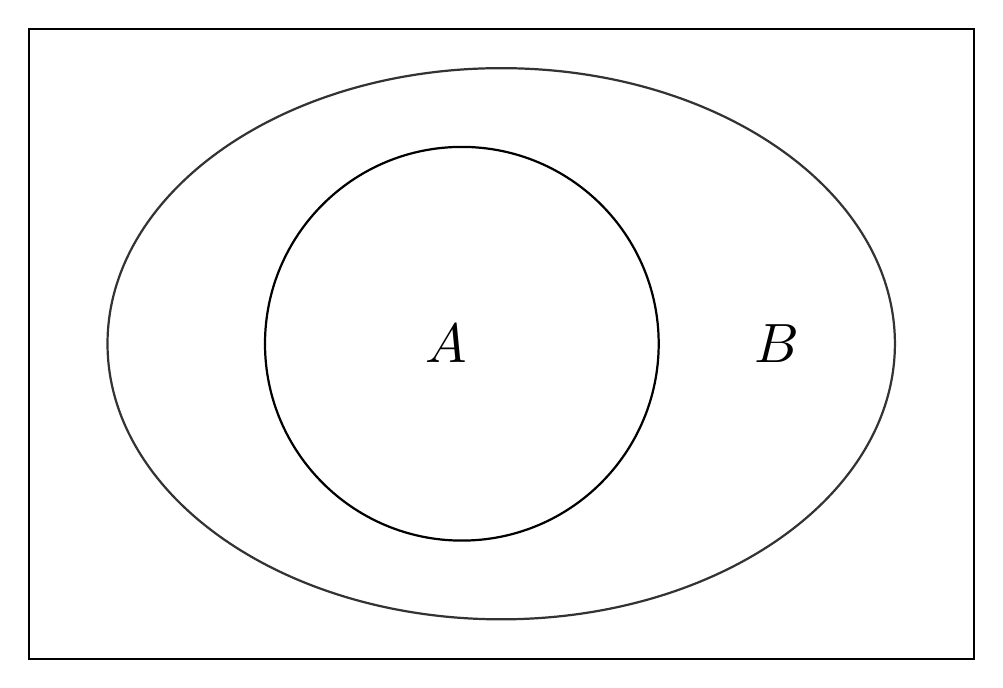
\begin{tikzpicture}[scale=2, transform shape] 
 
 \draw[draw=circle edge2, thick] (0,0) ellipse (2.5cm and 1.75cm);
 
\node at (-0.35,0) {$A$};
\node at (1.75,0) {$B$};
\draw[outline] \firstcircle;
%\draw[outline] \secondcircle;
 \draw[outline] \square; 
 % \node[anchor=south] at (current bounding box.north) {$P\wedge \neg P$};

\end{tikzpicture}
 
\end{document}
